\chapter{Power Management}
``It will also be interesting to look at Sapphire Rapids, which also implements Golden Cove cores, including an analysis of user space idle states, and AVX frequencies.''

\section{Infuence of Tiles}
\todoms{Where is the PMU?}

\section{Shared Frequency Domains}

\section{AVX Frequencies}

Starting with the Haswell Microarchitecture, Intel introduced the concept of AVX frequencies.~\cite{Hackenberg_2015_Haswell}
The concept has been extended with the Skylake Server Microarchitecture.
\todoms{cite Optimization Reference Manual: Volume 1 Section 2.6.3 SKYLAKE SERVER POWER MANAGEMENT}

Historically, instructions have been split into classes based on the used instruction set, i.e. AVX2 and AVX512.
With Ice Lake these classes have updated to better accomodate the actual power consumption of these operations.
\todoms{cite New 3rd Gen Intel® Xeon® Scalable Processor Codename: Ice Lake-SP}

With the addition of the AMX instruction set Intel split up these classes further into four classes.
\todoms{\url{https://www.servethehome.com/5th-gen-intel-xeon-scalable-emerald-rapids-resets-servers-by-intel/}}
In \todoms{cite Microarchitectural comparison and in-core modeling of state-of-the-art CPUs: Grace, Sapphire Rapids, and Genoa}, Laukemann et al. checked the CPU throttling for these classes however they we only able to show the throttling for classes \todoms{Class 0 and 1, verify this!}

\begin{figure}[]
    \centering
    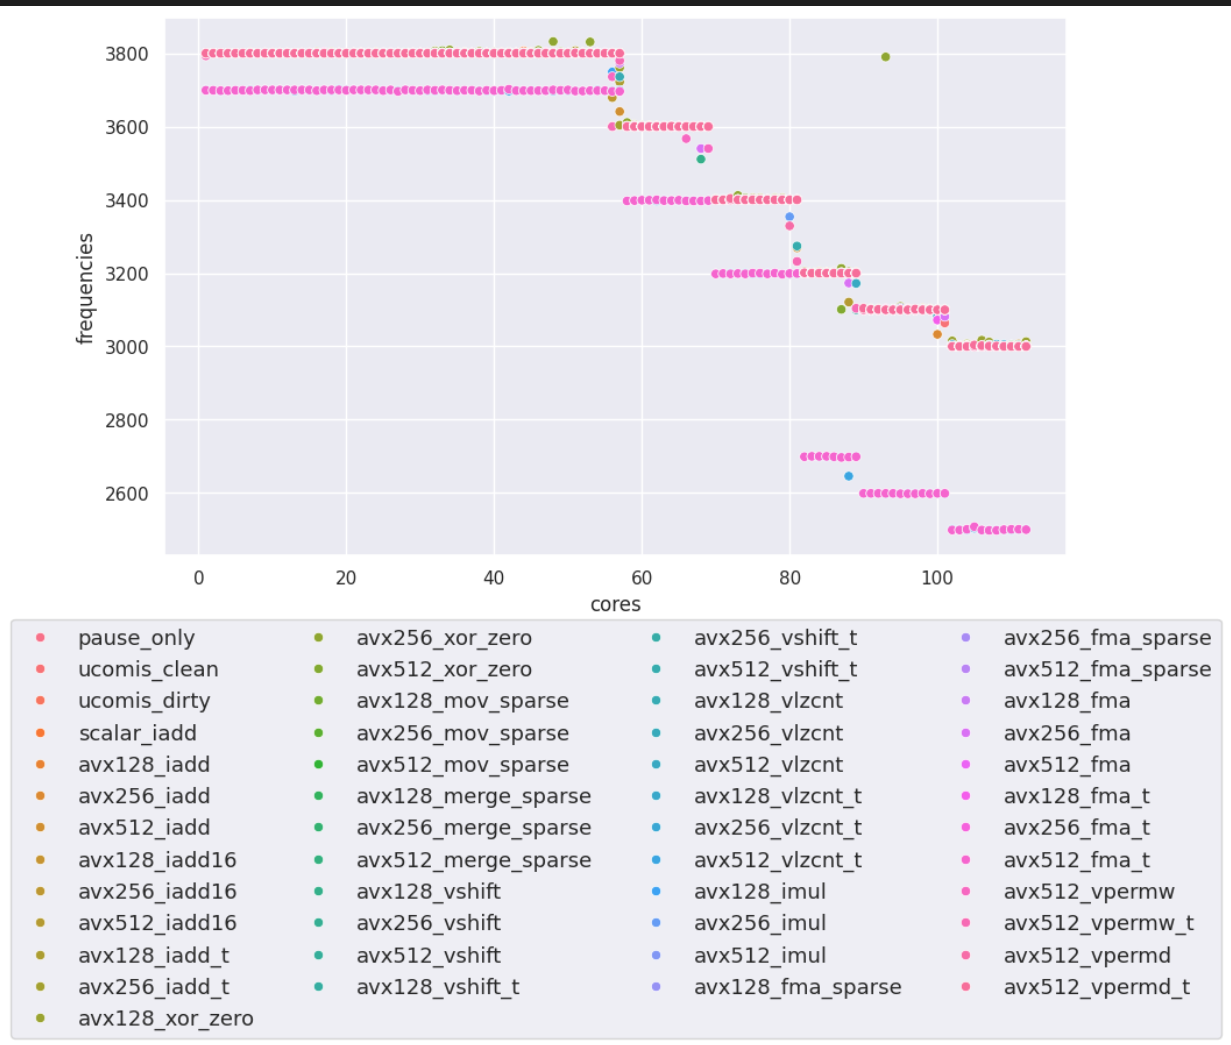
\includegraphics[width=0.8\columnwidth]{fig/turbo-frequencies-per-core.png}
    \caption{Reproduced figure from ...Microarchitectural comparison and in-core modeling of state-of-the-art CPUs: Grace, Sapphire Rapids, and Genoa... with avx-turbo}
\end{figure}



\todoms{Cdynn classes.}

\begin{table}[t]
	\centering
	\caption{\label{tab:cdyn-classes}AVX frequency classes based on published slides}
    \todoms{\url{https://www.servethehome.com/5th-gen-intel-xeon-scalable-emerald-rapids-resets-servers-by-intel/}}
	\begin{tabular}{|l|c|c|c|c|}
        \hline
        \diagbox[height=5em]{Instruction\\Class}{\\$C_{dyn}$ Class} & 0 & 1 & 2 & 3 \\
        \hline
        SSE & 128 Light & 128 Heavy & & \\
        AVX2 & 256 Light & 256 Moderate & 256 Heavy & \\
        AVX512 & 512 Ultra-Light & 512 Light & 512 Moderate & 512 Heavy \\
        AMX & & AMX Light & AMX Moderate & AMX Heavy \\
        \hline \hline
        Turbo Frequency & SSE & AVX2 & AVX512 & AMX \\ 
        \hline
	\end{tabular}
\end{table}

``smarter mapping between instructions and specific power levels'' See IceLakeSP Hotchips

\todoms{Reading the cdynn classes from the PMU (per core)}

\section{Uncore Frequency Scaling}

\section{Idle State Latencies}
\todoms{Both user and normal C states}